\documentclass[leqno]{article}
\usepackage{graphicx} % Required for inserting images
\usepackage[top=0.9in, bottom=1in, left=1.5in, right=1.5in]{geometry}
\usepackage[utf8]{inputenc}
\usepackage[icelandic]{babel}
\usepackage[T1]{fontenc}
\usepackage[parfill]{parskip}
% Tables and lists
\usepackage{booktabs,tabularx}
\usepackage{multirow}
\usepackage{enumerate}
\usepackage{adjustbox}
\usepackage{multicol}
\usepackage{xcolor}
\usepackage{algpseudocode}
\usepackage{tikz}
\usepackage{listings}
\lstset{
	basicstyle=\ttfamily,
	mathescape
}
\usetikzlibrary{arrows, positioning, calc, graphs}
\tikzset{
node distance=5mm,
>=stealth',
black!70,
text=black,
graphs/every graph/.style={edges=rounded corners},
vloop/.style={to path={-- ++(#1,0) |- (\tikztotarget)}},
hloop/.style={to path={-- ++($(0,0)-(#1,0)$) |- (\tikztotarget)}},
downright/.style={to path={-- ++(0.7,0) |- (\tikztotarget)}},
rightup/.style={to path={-- ++(1,0) |- (\tikztotarget)}},
hv path/.style={to path={-| (\tikztotarget)}},
vh path/.style={to path={|- (\tikztotarget)}},
box/.style={%
    rectangle,
    minimum size=6mm,
	rounded corners=1mm,
    draw=black,
    % Font
    %font=\itshape
},
start/.style={%
    circle,inner sep=1pt,minimum size=1pt,fill=white,draw=black!70,text=black!70
},
end/.style={%
    start, draw=black,text=black,
},
junction/.style={circle,inner sep=0pt,minimum size=0pt},
}


% Math
\usepackage{amsmath, amssymb}
% Graphics

\usepackage{graphicx}
% Code environment
\usepackage{minted}

\renewcommand\thesubsection{}

\title{Forritunarmál Verkefni 1}
\author{Ragnar Björn Ingvarsson, rbi3}


\begin{document}
	
	\maketitle

	\newpage
	
	\part{Hópverkefni}

	\section{Hvað er mál?}

	Svarið hér er \textbf{(B)}, Mengi strengja.

	\section{Sýnið BNF, EBNF og málrit fyrir eftirfarandi mál}

	\subsection{a) $\{a^nb^kc^n|n,k \in \mathbb{N}\}$}

		\begin{center}\begin{tabular}{rl}
				\textbf{BNF:} &
			\begin{lstlisting}
<R> ::= 'a' <R> 'c' | <B>
			\end{lstlisting} \\
							  & \begin{lstlisting}
<B> ::= 'b' <B> | $\lambda$ 
			  \end{lstlisting} \\[5ex]

				\textbf{EBNF:} &
			\begin{lstlisting}
R = 'a', R, 'c' | {'b'};
			\end{lstlisting} \\[5ex]
				\textbf{Málrit:} &
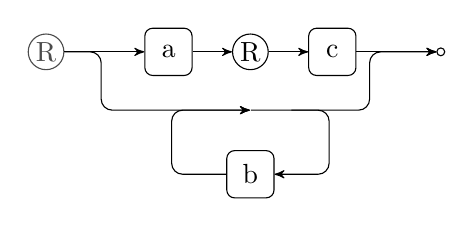
\begin{tikzpicture}

\node[start] (start) {R};
\node[junction,right=of start] (p1) {};
\node[box,right=of p1] (a) {a};
\node[end,right=of a] (R) {R};
\node[box,right=of R] (c) {c};
\node[junction,below=of R] (b) {};
\node[junction,right=of c] (p2) {};
\node[end,right=of p2] (end) {};
\node[junction,left=of b] (p3) {};
\node[box,below=of b] (p4) {b};
\node[junction,right=of b] (p5) {};

\graph [use existing nodes] {
start -> a -> R -> c -> end;
start ->[downright] b;
p5 ->[rightup] end;
b ->[vloop] p4;
p4 ->[hloop] b;
};

\end{tikzpicture} \\


		\end{tabular}
	\end{center}

		\subsection{b) $\{(ab)^nc^kd^k|n,k \in \mathbb{N}\}$}

		\begin{center}\begin{tabular}[t]{rl}
				\textbf{BNF:} &
			\begin{lstlisting}
<R> ::= <abpart> <cdpart>
			\end{lstlisting} \\
							  & \begin{lstlisting}
<abpart> ::= 'ab' <abpart> | $\lambda$
			\end{lstlisting} \\
							  & \begin{lstlisting}
<cdpart> ::= 'c' <cdpart> 'd' | $\lambda$
			\end{lstlisting} \\[5ex]

				\textbf{EBNF:} &
			\begin{lstlisting}
R = {'ab'}, cdpart;
			\end{lstlisting} \\
							  & \begin{lstlisting}
cdpart = ['c', cdpart, 'd'];
			\end{lstlisting} \\[8ex]

				\textbf{Málrit:} &

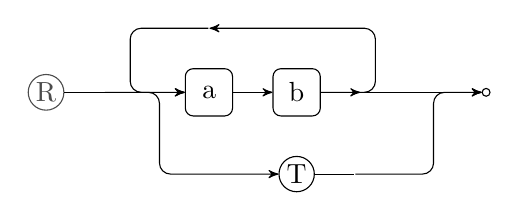
\begin{tikzpicture}
	\node[start, text=black!70] (start) {R};
	\node[junction, right=of start] (p1) {};
	\node[junction, right=of p1] (p2) {};
	\node[box, right=of p2] (a) {a};
	\node[box, right=of a] (b) {b};
	\node[junction, right=of b] (p3) {};
	\node[junction, right=of p3] (p4) {};
	\node[junction, right=of p4] (p6) {};
	\node[end, right=of p6] (end) {};
	\node[end, below=of b] (cdpart) {T};
	\node[junction, above=of a] (p5) {};
	\node[junction, right=of cdpart] (p7) {};


\graph [use existing nodes] {
start -> a -> b -> p3 -> end;
p1 ->[downright] cdpart;
cdpart -- p7 ->[rightup] end;
b ->[vloop] p5;
p5 ->[hloop] a;
};

\end{tikzpicture} \\ \\
& 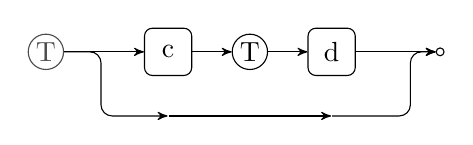
\begin{tikzpicture}
	\node[start, text=black!70] (start) {T};
	\node[junction, right=of start] (p1) {};
	\node[box, right=of p1] (c) {c};
	\node[end, right=of c] (T) {T};
	\node[box, right=of T] (d) {d};
	\node[junction, right=of d] (p2) {};
	\node[end, right=of p2] (end) {};
	\node[junction, below=of c] (p3) {};
	\node[junction, below=of d] (p4) {};

\graph [use existing nodes] {
start -> c -> T -> d -> end;
start ->[downright] p3;
p3 -> p4;
p4 ->[rightup] end;
};
\end{tikzpicture}

			\end{tabular}
		\end{center}

	\subsection{c) $\{a^nb^nc^n|n \in \mathbb{N}\}$}

		\begin{center}\begin{tabular}{rl}
				\textbf{BNF:} &
				Impossible \\[5ex]

				\textbf{EBNF:} &
				Impossible \\[5ex]

				\textbf{Málrit:} &
				Impossible \\[5ex]
			\end{tabular}
		\end{center}

		\subsection{d) $\{a^nb^nc^k|n,k \in \mathbb{N}\}$}

		\begin{center}\begin{tabular}{rl}
				\textbf{BNF:} &
			\begin{lstlisting}
<R> ::= <abpart> <cpart>
			\end{lstlisting} \\
							  & \begin{lstlisting}
<abpart> ::= 'a' <abpart> 'b' | $\lambda$
			\end{lstlisting} \\
							  & \begin{lstlisting}
<cpart> ::= 'c' <cpart> | $\lambda$
							  \end{lstlisting} \\[5ex]

				\textbf{EBNF:} &
			\begin{lstlisting}
R = abpart, {'c'};
			\end{lstlisting} \\
							  & \begin{lstlisting}
abpart = ['a', abpart, 'b'];
							  \end{lstlisting} \\[5ex]

				\textbf{Málrit:} & 
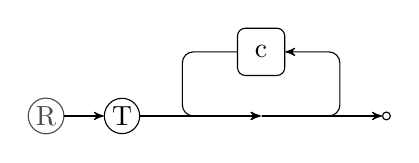
\begin{tikzpicture}
	\node[start] (start) {R};
	\node[end, right=of start] (T) {T};
	\node[junction, right=of T] (p) {};
	\node[junction, right=of p] (p1) {};
	\node[junction, right=of p1] (c) {};
	\node[junction, right=of c] (p2) {};
	\node[box, above=of c] (p3) {c};
	\node[junction, right=of p2] (p4) {};
	\node[end, right=of p4] (end) {};

\graph [use existing nodes] {
start -> T -> c -> end;
c ->[vloop] p3;
p3 ->[hloop] c;
};
\end{tikzpicture} \\ \\
& 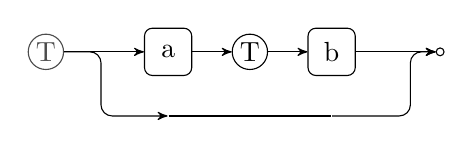
\begin{tikzpicture}
	\node[start] (start) {T};
	\node[junction, right=of start] (p1) {};
	\node[box, right=of p1] (a) {a};
	\node[end, right=of a] (T) {T};
	\node[box, right=of T] (b) {b};
	\node[junction, right=of b] (p2) {};
	\node[junction, below=of a] (p3) {};
	\node[junction, below=of b] (p4) {};
	\node[end, right=of p2] (end) {};

\graph [use existing nodes] {
start -> a -> T -> b -> end;
start ->[downright] p3 -- p4 ->[rightup] end;
};
\end{tikzpicture} \\[5ex]
			\end{tabular}
		\end{center}


		\section{Lýsið því máli sem BNF-mállýsingin skilgreinir}
		\[
			\langle x \rangle ::= x  \langle x \rangle
		\]\[
		\hspace{1em} | \hspace{1em} \langle y \rangle
		\]
		\[
			\langle y \rangle ::= y  \langle y \rangle
		\]\[
		\hspace{.2em} | \hspace{1em} \lambda
		\]


		Við sjáum að BNF-mállýsingin myndi vera skrifuð sem $x^*y^*$ með 
		reglulegri segð og við getum þá lýst málinu sem óákveðið mörg x, 
		fylgd eftir af óákveðið mörgum y.

		Málrit væri þá svoleiðis:

		\begin{center}
		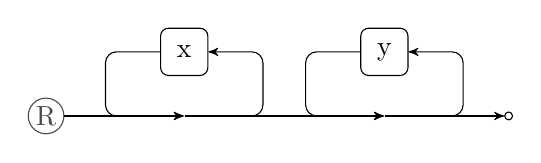
\begin{tikzpicture}
			\node[start] (start) {R};
			\node[junction, right=1 of start] (p1) {};
			\node[junction, right=of p1] (x) {};
			\node[junction, right=1.5 of x] (p2) {};
			\node[junction, right=of p2] (p3) {};
			\node[junction, right=of p3] (y) {};
			\node[junction, right=of y] (p4) {};
			\node[end, right=1 of p4] (end) {};
			\node[box, above=of x] (x1) {x};
			\node[box, above=of y] (y1) {y};

			\graph [use existing nodes] {
				start -> x -> y -> end;
				x ->[vloop] x1 ->[hloop] x;
				y ->[vloop] y1 ->[hloop] y;
			};
		\end{tikzpicture}
		\end{center}

		Og á sama hátt væri endanleg stöðuvél nokkurnveginn svona:

		\begin{center}
			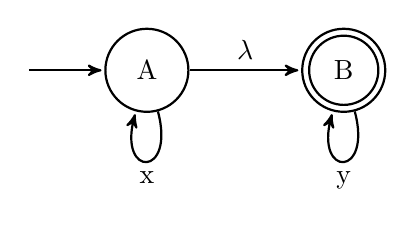
\begin{tikzpicture}[->, >=stealth', shorten >=1pt, auto, node distance=2cm,thick, main node/.style={circle,draw,minimum size=3em}]
				 
				\node[main node] at (1.5,0) (a) {A};
				\node[main node] at (4,0) (b) {B};
				\node[main node, minimum size=2.5em] at (4,0) (bfin) {};


			\path (a) edge node {$\lambda$} (b);
			\path (a) edge [loop below=60] node {x} (a);
			\path (b) edge [loop below=60] node {y} (b);
			\path (0,0) edge node {} (a);

			\end{tikzpicture}
		\end{center}

		\tikzset{->, >=stealth', shorten >=1pt, auto, node distance=2cm,thick, main node/.style={circle,draw,minimum size=3em}}
				 


		\part{Einstaklingsverkefni}
		\setcounter{section}{0}
		\section{Hverjar af fullyrðingunum eru réttar?}

		\section{Hvaða mállýsingar lýsa reglulegu máli?}

\vspace{2em}

		\begin{itemize}
\begin{minipage}{.20\linewidth}
			\item[a)]$\begin{alignedat}{3}
\langle & x & \rangle :& \hspace{-.3em}:= & x & \langle x \rangle \\
		&   &          &  |               & \langle & y \rangle \\
\langle & y & \rangle :& \hspace{-.3em}:= & y & \langle y \rangle \\
		&   &          &  |               & \langle & z \rangle \\
\langle & z & \rangle :& \hspace{-.3em}:= & z & \langle z \rangle \\
		&   &          &  |               & \langle & x \rangle \\
		&   &          &  |               & \epsilon & \\
\end{alignedat}$\end{minipage}\begin{minipage}{.80\linewidth}
Þessi mállýsing lýsir reglulegu máli sem getur verið lýst með \\ reglulegu segðinni $(x^*y^*z^*)^*$ og þá með endanlegu stöðuvélinni:
\\
\begin{center}
\begin{tikzpicture}
	\node[main node] (A) {A};
	\node[main node] at (2.5,0) (B) {B};
	\node[main node] at (5,0) (C) {C};
	\node[main node, minimum size=2.5em] at (5,0) (Cfin) {};


	\path (A) edge node {$\lambda$} (B);
	\path (B) edge node {$\lambda$} (C);
	\path (A) edge [loop above=60] node {x} (A);
	\path (B) edge [loop above=60] node {y} (B);
	\path (C) edge [loop above=60] node {z} (C);
	\path (C) edge [bend left=35] node {$\lambda$} (A);
	\path (-1,0) edge node {} (A);
\end{tikzpicture}
\end{center}
\end{minipage}

\vspace{3em}

\begin{minipage}{.20\linewidth}
			\item[b)] $\begin{alignedat}{3}
\langle & x & \rangle :& \hspace{-.3em}:= & x & \langle x \rangle \\
		&   &          &  |               & \langle & y \rangle \\
\langle & y & \rangle :& \hspace{-.3em}:= & y & \langle y \rangle \\
		&   &          &  |               & \langle & z \rangle \\
\langle & z & \rangle :& \hspace{-.3em}:= & z & \langle z \rangle \\
		&   &          &  |               & \epsilon & \\
    \end{alignedat}$
\end{minipage}
\begin{minipage}{.80\linewidth}
	Þessi mállýsing lýsir einnig reglulegu máli sem getur verið lýst \\
	með reglulegu segðinni $x^*y^*z^*$ sem við setjum upp í endanlega
	 stöðuvél svona:
	 \\
\begin{center}
	\begin{tikzpicture}
	\node[main node] (A) {A};
	\node[main node] at (2.5,0) (B) {B};
	\node[main node] at (5,0) (C) {C};
	\node[main node, minimum size=2.5em] at (5,0) (Cfin) {};


	\path (A) edge node {$\lambda$} (B);
	\path (B) edge node {$\lambda$} (C);
	\path (A) edge [loop above=60] node {x} (A);
	\path (B) edge [loop above=60] node {y} (B);
	\path (C) edge [loop above=60] node {z} (C);
	\path (-1,0) edge node {} (A);
	\end{tikzpicture}
\end{center}
\end{minipage}

\vspace{3em}

\begin{minipage}{.20\linewidth}
			\item[c)] $\begin{alignedat}{3}
\langle & x & \rangle :& \hspace{-.3em}:= & \langle & x \rangle + \langle x \rangle \\
		&   &          &  |               & (\langle & x \rangle) \\
		&   &          &  |               & & x \\
    \end{alignedat}$
\end{minipage}
\begin{minipage}{.80\linewidth}
	Þessi mállýsing lýsir ekki reglulegu máli þar sem ekki er hægt að 
	gera ráð fyrir öllum mögulegum samsetningum af svigum sem geta myndast
	 hér. Ómögulegt er þá að búa til reglulega segð og einnig endanlega 
	 stöðuvél
 \end{minipage}

 \vspace{3em}

 \begin{minipage}{.20\linewidth}
			\item[d)] $\begin{alignedat}{3}
\langle & x & \rangle :& \hspace{-.3em}:= & \langle & x \rangle + \langle x \rangle \\
		&   &          &  |               & & x \\
    \end{alignedat}$
\end{minipage}
\begin{minipage}{.80\linewidth}
	Þessi mállýsing lýsir hins vegar reglulegu máli sem getur verið skrifað 
	sem reglulega segðin $(x+)^*x$ með endanlegu stöðuvélina:

\vspace{1.5em}

\begin{center}
	\begin{tikzpicture}
	\node[main node] (A) {A};
	\node[main node] at (2.5,0) (B) {B};
	\node[main node, minimum size=2.5em] at (2.5,0) (Cfin) {};


	\path (A) edge node {x} (B);
	\path (A) edge [loop below=60] node {x+} (A);
	\path (-1,0) edge node {} (A);
	\end{tikzpicture}
\end{center}
\end{minipage}

\vspace{3em}

\begin{minipage}{.20\linewidth}
			\item[e)] $\begin{alignedat}{3}
\langle & x & \rangle :& \hspace{-.3em}:= & (\langle & x \rangle)  \langle x \rangle \\
		&   &          &  |               & & \epsilon \\
    \end{alignedat}$

\end{minipage}
\begin{minipage}{.80\linewidth}

	Þessi mállýsing lýsir ekki reglulegu máli af sömu ástæðu og c), ekki er 
	hægt að gera ráð fyrir öllum mögulegum samsetningum sviga. Hvorki er þá 
	hægt að að skrifa reglulega segð né teikna endanlega stöðuvél.

\end{minipage}

\vspace{3em}

\begin{minipage}{.20\linewidth}
			\item[f)] $\begin{alignedat}{3}
\langle & x & \rangle :& \hspace{-.3em}:= & \langle & x \rangle  \langle x \rangle +\\
		&   &          &  |               & & x \\
    \end{alignedat}$
\end{minipage}
\begin{minipage}{.80\linewidth}
	Þessi mállýsing lýsir reglulegu máli sem getur verið lýst með 
	reglulegri segð á þennan máta: $x(x^++^+)*$. Svo lítur endanlega 
	stöðuvélin svona út:

	\begin{tikzpicture}
		\node[main node] (A) {A};
		\node[main node] at (2.5,0) (B) {B};
		\node[main node] at (5,0) (C) {C};
		\node[main node] at (7.5,0) (D) {D};
		\node[main node, minimum size=2.5em] at (7.5,0) (Dfin) {};

		\path (A) edge node {x} (B);
		\path (B) edge node {x} (C);
		\path (C) edge node {+} (D);
		\path (B) edge [loop above=60] node {x} (B);
		\path (C) edge [loop above=60] node {+} (C);
		\path (C) edge [bend left=55] node {$\lambda$} (B);
		\path (A) edge [bend right=55] node {x} (D);
		\path (-1,0) edge node {} (A);
	\end{tikzpicture}
\end{minipage}
\end{itemize}

\newpage
\section{Sýnið BNF fyrir \{x,y\} þar sem x er slétt tala}

Við skrifum fyrst reglulega segð fyrir þetta og hún kemur út sem: 
$y^*(xy^*xy^*)^*$. Við getum svo breytt henni í BNF og við fáum:
\begin{lstlisting}
		  <R> ::= <R> x <R> x <R> | <Y>
		  	<Y> ::= y <Y> | $\lambda$
\end{lstlisting}

Og svo endanleg stöðuvél lítur svona út:

\begin{center}
	\begin{tikzpicture}
		\node[main node] (A) {A};
		\node[main node] at (2.5,0) (B) {B};
		\node[main node, minimum size=2.5em] (Afin) {};

		\path (A) edge [bend left=30] node {x} (B);
		\path (A) edge [loop above=60] node {y} (A);
		\path (B) edge [loop above=60] node {y} (B);
		\path (B) edge [bend left=30] node {x} (A);
		\path (-1,0) edge node {} (A);
	\end{tikzpicture}
\end{center}

Einnig myndi þá útleiðslutré fyrir strenginn xyyx með þessu BNF vera svo:

\begin{center}
\begin{tikzpicture}[-, cube/.style={box,draw=white, thick}]
	\node[cube] at (0,0.5) (start) {\texttt{<R>}};
	\node[cube] at (-3.5,-1) (1R1) {\texttt{<R>}};
	\node[cube] at (-2,-1) (1x1) {\texttt{x}};
	\node[cube] at (0,-1) (1R2) {\texttt{<R>}};
	\node[cube] at (2,-1) (1x2) {\texttt{x}};
	\node[cube] at (3.5,-1) (1R3) {\texttt{<R>}};

	\node[cube] at (-3.5,-2) (2Y1) {\texttt{<Y>}};
	\node[cube] at (0,-2) (2Y2) {\texttt{<Y>}};
	\node[cube] at (3.5,-2) (2Y3) {\texttt{<Y>}};

	\node[cube] at (-3.5,-3) (3l1) {$\lambda$};
	\node[cube] at (-1.2,-3) (3y1) {\texttt{y}};
	\node[cube] at (1.2,-3) (3Y1) {\texttt{<Y>}};
	\node[cube] at (3.5,-3) (3l2) {$\lambda$};

	\node[cube] at (0.8,-4) (4y1) {\texttt{y}};
	\node[cube] at (1.6,-4) (4Y1) {\texttt{<Y>}};

	\node[cube] at (1.6,-5) (5l1) {$\lambda$};

	\path (start) edge node {} (1R1);
	\path (start) edge node {} (1x1);
	\path (start) edge node {} (1R2);
	\path (start) edge node {} (1x2);
	\path (start) edge node {} (1R3);

	\path (1R1) edge node {} (2Y1);
	\path (1R2) edge node {} (2Y2);
	\path (1R3) edge node {} (2Y3);

	\path (2Y1) edge node {} (3l1);
	\path (2Y2) edge node {} (3y1);
	\path (2Y2) edge node {} (3Y1);
	\path (2Y3) edge node {} (3l2);

	\path (3Y1) edge node {} (4y1);
	\path (3Y1) edge node {} (4Y1);

	\path (4Y1) edge node {} (5l1);
\end{tikzpicture}
\end{center}

\section{Sýnið BNF o.fl. fyrir mál með $a$, $+$ og svigum}

Sjáum útfrá löglegum dæmum sem voru tekin fyrir að BNF myndi líta svo út:
\begin{lstlisting}
		 <R> ::= a | (<R>) | <R> + <R>
\end{lstlisting}
Svo er EBNF svona:
\begin{lstlisting}
		 R = a | (, R, ) | R, +, R;
\end{lstlisting}

Og loks lítur málrit fyrir þetta mál segða svona út:


\tikzset{
node distance=5mm,
>=stealth',
black!70,
text=black,
graphs/every graph/.style={edges=rounded corners},
vloop/.style={to path={-- ++(#1,0) |- (\tikztotarget)}},
hloop/.style={to path={-- ++($(0,0)-(#1,0)$) |- (\tikztotarget)}},
downright/.style={to path={-- ++(0.7,0) |- (\tikztotarget)}},
rightup/.style={to path={-- ++(1,0) |- (\tikztotarget)}},
hv path/.style={to path={-| (\tikztotarget)}},
vh path/.style={to path={|- (\tikztotarget)}},
box/.style={%
    rectangle,
    minimum size=6mm,
	rounded corners=1mm,
    draw=black,
    % Font
    %font=\itshape
},
start/.style={%
    circle,inner sep=1pt,minimum size=1pt,fill=white,draw=black!70,text=black!70
},
end/.style={%
    start, draw=black,text=black,
},
junction/.style={circle,inner sep=0pt,minimum size=0pt},
}

\begin{center}
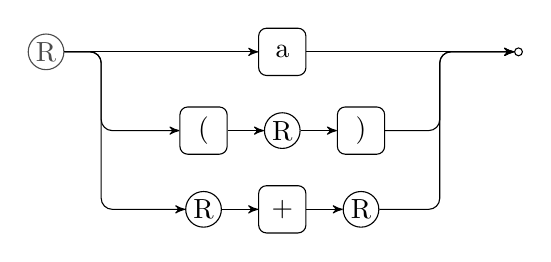
\begin{tikzpicture}
	\node[start] (start) {R};
	\node[junction] at (1,0) (p1) {};
	\node[box] at (3,0) (a) {a};
	\node[junction] at (5,0) (p2) {};
	\node[end] at (6,0) (end) {};
	\node[junction] at (1,-1) (p3) {};
	\node[box] at (2,-1) (Lpar) {(};
	\node[end] at (3,-1) (R1) {R};
	\node[box] at (4,-1) (Rpar) {)};
	\node[junction] at (5,-1) (p4) {};
	\node[junction] at (1,-2) (p5) {};
	\node[end] at (2,-2) (R2) {R};
	\node[box] at (3,-2) (+) {+};
	\node[end] at (4,-2) (R3) {R};
	\node[junction] at (5,-2) (p6) {};

	\graph [use existing nodes] {
	start -> a -> end;
	start ->[downright] Lpar;
	Lpar -> R1 -> Rpar;
	Rpar ->[rightup] end;
	start ->[downright] R2;
	R2 -> + -> R3;
	R3 ->[rightup] end;
	};

\end{tikzpicture}
\end{center}

\end{document}
